\chapter{Data}

\section{Grammatical inflection data}

In order to assess grammatical similarities between languages, the data set published for the SIGMORPHON first shared task 2019, a subset of the data set for the first SIGMORPHON 2018 shared task, was used. Both sets are publicly available on GitHub (\cite{McCarthy2019}, \cite{Cotterell2018b}).

The first 2018 shared task was simply a morphology learning problem. The data consists of triples - lemma, target grammatical category values, and correctly inflected form - for 103 languages, partitioned into training, development, and test sets. An example of some Finnish triples is shown in Fig. \ref{fig:fintrip}. The training sets are further partitioned into low, medium, and high-resource sets; the low-resource training sets contain about 100 forms, medium about 1,000 forms, and high about 10,000 forms, with the sets being nested so that the smaller training sets are subsets of the larger ones. These data levels are used to simulate different resource settings, e.g., low-resource training sets represent data available for a poorly-resourced language; the data levels can also be used to assess model learning curve \parencite{Cotterell2018b}.

The 2019 shared task was a transfer learning task, which sought to use a large volume of data about a source language to inform a model with access to a low volume of data for the target language. The data available for the task was a subset of the 2018 data. The task consisted of 100 pairs across 79 languages. For each training pair, some data sets from 2018 were used: the high-resource training data for the source language and the low-resource training set and development and test data sets for the target language \parencite{McCarthy2019}.

\begin{figure}[ht]
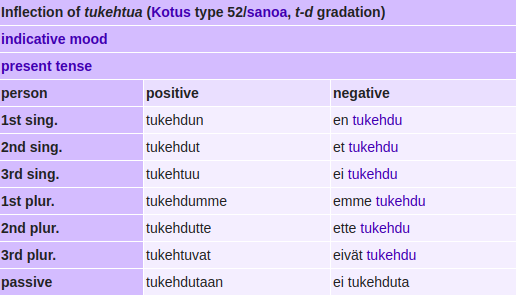
\includegraphics[width=12cm]{images/tukehtua.png}
\centering
\caption{The English Wiktionary partial inflection table for the Finnish word \textit{tukehtua}.}
\label{fig:wikt}
\end{figure}

\begin{figure}[ht]
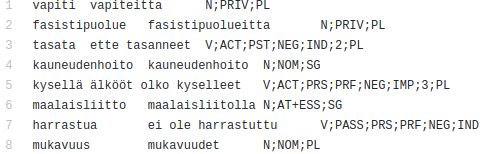
\includegraphics[width=12cm]{images/sigmorphon2018_fn.png}
\centering
\caption{A sample of the SIGMORPHON 2018 data for Finnish, \\
scraped from Wiktionary and provided on GitHub\\ (https://github.com/sigmorphon/conll2018/blob/master/task1/all/finnish-train-high).}
\label{fig:fintrip}
\end{figure}

\subsection{Language diversity}

The languages represented in the 2018 data cover a wide range of families and typological categories. Although over half of the languages are from the Indo-European family, a grouping that includes most languages of Europe, Greater Iran, and the northern part of the Indian subcontinent, one or more languages each of the Athabaskan, Bantu, Causasian, Kartvelian, Quechua, Semitic, Sino-Tibetan, Turkic, and Uralic families, as well as two isolates (Haida and Basque), are represented. Diverse inflection strategies are also represented, including suffixing, prefixing, infixing, ablaut, and introflexion, and long-distance processes like vowel harmony and consonant harmony \parencite{Cotterell2018b}. 

Among the 2019 pairs, all the aforementioned families except Athabaskan, Kartvelian, and Sino-Tibetan are represented \parencite{McCarthy2019}. The pairs are not chosen randomly from among the 2018 languages; many languages are chosen more often as source than target languages and vice versa, and the Turkic language family in particular was exhaustively paired. I conjecture that many seemingly difficult-to-explain trends in the data are related to confounding factors in the choices of language pairs, and in the conclusion section I will discuss what some of these effects may be and how future work might overcome these confounds.

\subsection{Sourcing and sampling}

The English Wiktionary, a collaborative online dictionary, has become something of a standard source of supervised morphological data (\cite{Cotterell2016}, \cite{Cotterell2017a}, \cite{Cotterell2018b}). It provides full or partial inflection tables alongside lexeme definitions; the structure of tables is consistent for a given language and part of speech. An example table is given in Fig. \ref{fig:wikt}. For some highly inflected languages (e.g., Navajo), Wiktionary only provides a fixed subset of forms. For some relationships between words that could be considered grammatical, it may simply offer them as separate lexical entries; for example, Russian perfect and imperfect forms are given as separate entries, as are Navajo verb forms that vary by aspect or thematic classifier \parencite{Wiktionary}.  

For most of the languages in the SIGMORPHON 2018 data, forms were gathered via scraping from Wiktionary. Multiple parts of speech are represented for most languages, but only parts of speech with a significant number of entries relative to all entries in a given language. Inflected forms were sampled for inclusion according to their estimated distribution in the text of Wikipedia for each respective language. For languages with sufficient data, 12,000 forms were sampled, and from these 1,000 were randomly selected for the development set and 1,000 for the testing set; the remaining 10,000 became the high-resource training set, of which 1,000 were randomly chosen as the medium-resource set and 100 of those as the low-resource set. For languages with less available data, sets might be smaller and the high-resource training set might be omitted; 17 languages lack high-resource sets \parencite{Cotterell2018b}.

\subsection{Representation of morphology}

The SIGMORPHON data set uses the UniMorph format to indicate grammatical categories  \parencite{Cotterell2018b}. The UniMorph project, initially published in 2015, is a format for encoding morphological categories uniformly cross-linguistically. It uses a universal label set to encode morphological categories across languages. An example of the annotation can be seen in Fig. \ref{fig:fintrip}, where words are marked for, e.g., part of speech (\texttt{ADJ, V, N}), voice (\texttt{PASS}), tense (\texttt{PRS}), number (\texttt{SG, PL}), and other categories (\cite{SylakGlassman2015}, \cite{SylakGlassman2015a}, \cite{SylakGlassman2016}). These annotations were key in generating important metrics of language pairs for this study: category overlap for each part of speech, and part of speech distribution similarity, discussed in sections \ref{sec:CO} and \ref{sec:POSDS} respectively.

\section{Language typology and genealogy data}

Data about language typology was drawn from the World Atlas of Language Structures (WALS), Ethnologue, and generated from the UniMorph tags in the SIGMORPHON 2019 data.

\subsection{Typology data from WALS}

The World Atlas of Language Structures is "a large database of structural (phonological, grammatical, lexical) properties of languages gathered from descriptive materials (such as reference grammars) by a team of 55 authors." It contains information about twelve morphology features, such as "Reduplication," "Prefixing vs. Suffixing in Inflectional Morphology," and "Inflectional Synthesis of the Verb" \parencite{WALS}. WALS labels for twelve morphological features were scraped and collected for all languages for which they are currently available. Among the 79 languages present in the SIGMORPHON 2019 transfer pairs, as many as 47 had labels available for a particular feature ("Prefixing vs. Suffixing in Inflectional Morphology"), while as few as 17 had labels available for other features ("Fusion of Selected Inflectional Formatives", "Exponence of Selected Inflectional Formatives", "Exponence of Tense-Aspect-Mood Inflection"). The full set of scraped data can be found on the GitHub repository for this paper; explanations of the categories can be found on WALS. 

Some of these may also be measurable via analysis of the SIGMORPHON data as well, e.g., "Exponence of Tense-Aspect-Mood Inflection," "Prefixing vs. Suffixing in Inflectional Morphology," and "Case Syncretism," while others, such as "Reduplication" and "Locus of Marking in the Clause" would probably be harder to measure in such a way. For the features which can also be generated by looking at the SIGMORPHON data, the WALS data can at least be used as a gold standard to calibrate and assess the quality of generated metrics. WALS will not be useful in assessing overlap between sets of inflectional categories which are present or exhibit fusion in languages - its categorical tagging is simply not granular enough - but fortunately these will be relatively straightforward measures to generate from the SIGMORPHON 2018 data.

\begin{figure}[ht]
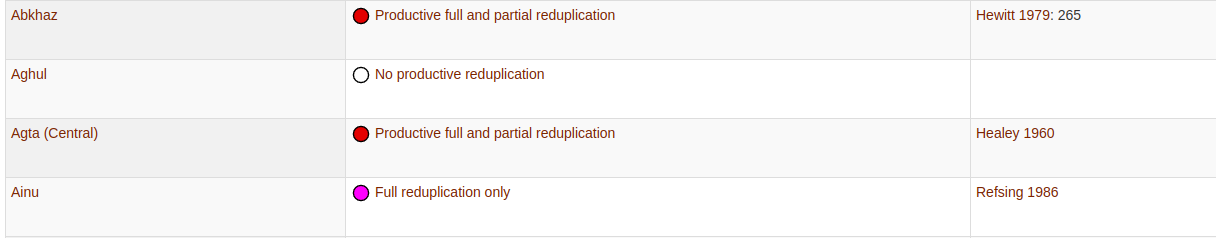
\includegraphics[width=13.5cm]{images/WALS.png}
\centering
\caption{A sample of WALS data on reduplication, available at\\ https://wals.info/feature/27A, accessed 19 Nov 2019.}
\end{figure}

\subsection{Genealogy from Ethnologue}

SIGMORPHON 2018 supplied a basic "Family" designation for each of the 103 languages in its data set, but these do not correspond to any particular taxonomic level; some, such as Indo-European and Uralic, are language families, the most broad designation of language genealogy, while others, like Semitic, Slavic, and Romance, are subfamilies of various size. Language genealogy data from Ethnologue, a database of basic typological and socioliguistic information about all recognized languages, was used to supplement the SIGMORPHON 2018 labels and provide a more fine-grained measure of distance of relation between languages; my designations can be found on the GitHub repository for this paper \parencite{Ethnologue}.

\subsection{Part of speech category sets}

As a simple measure of language structure, the SIGMORPHON 2019 data was scraped for UniMorph tags to identify the total set of morphological tags present for each language and each part of speech. For instance, the set of tags found on German nouns is \texttt{ACC;DAT;GEN;NOM;PL;SG}. This measure should not be taken as a set of all inflectional categories actually used in a particular language; the SIGMORPHON data can skew toward particular parts of speech or particular inflection types. The generated category sets were simply used as a rudimentary measure of structural similarity between languages. For instance, if a language A marks nouns for case but not definiteness, then another language B that marks nouns for case as well is in some sense more similar to language A than a language C that does not mark case but does mark definiteness on nouns.

\section{Model performance data}

\subsection{SIGMORPHON 2018}

For the SIGMORPHON 2018 shared task 1, a morphological inflection task that did not license transfer learning, 27 models were submitted. Each model was described in a separate paper. In an appendix, SIGMORPHON 2018 published detailed results of the accuracy of each model on each language in low, medium, and high-resource settings, allowing for analysis of the specific performance differences of those models.

\subsection{SIGMORPHON 2019}

For the SIGMORPHON 2019 shared task 1, 13 models were submitted. Only two teams described their submissions in separately published papers; of those, only one published detailed data about the performance of its model on each transfer pair. SIGMORPHON 2019 only published average accuracy and Levenshtein distance of each team's submission, and the accuracy and Levenshtein distance of the baseline and highest-scoring submission for each transfer pair, so detailed comparison of the performance of each model was not possible.

\section{A note on publishing}

I have elected not to include my generated data in an appendix to this paper. Please find it online at \texttt{https://github.com/cstuartroe/thesis/tree/master/csv}.